
\documentclass[prd,onecolumn,showpcs,amsmath,amssymb,nofootinbib,notitlepage,preprintnumbers,balancelastpage,longbibliography]{revtex4-2}
\usepackage{tikz}
\usepackage{tikz-feynman}

\usepackage{amsfonts}
\usepackage{amsmath}
\usepackage{hyperref}
\hypersetup{breaklinks=true, colorlinks=true, citecolor=blue, linkcolor=blue, urlcolor=blue,filecolor=blue}
\usepackage{anyfontsize}
 \usepackage{booktabs}
\usepackage{ulem}
\usepackage{lineno}
\usepackage{cancel}
\usepackage[utf8]{inputenc}
\usepackage{multirow}
\usepackage{mathrsfs}
\usepackage{feynmp}
\usepackage{amsmath,amssymb,amsthm,amsfonts}
\usepackage{braket}
%\usepackage{subfigure}
%\usepackage{dcolumn}	% Align table columns on decimal point
%\usepackage{bm}		% bold math
%\usepackage{epsfig}
%\usepackage{epstopdf}
\usepackage{setspace}
\usepackage{datetime}
\usepackage{comment}

\usepackage{titlesec, titletoc}
\usepackage{latexsym}
\usepackage{slashed}
%\usepackage{caption}
\pagenumbering{arabic}

\usepackage{graphicx}
\usepackage{subcaption}
%\usepackage{floatrow}
%\usepackage{subfig}
%\usepackage[final]{graphicx}

\usepackage{calc}

\usepackage{graphicx}% Include figure files
\usepackage{dcolumn}% Align table columns on decimal point
\usepackage{bm}% bold math
\usepackage{epsfig}
%\usepackage[usenames]{color}
%\usepackage[usenames, dvipsnames]{color}
\usepackage{slashed}
\newcommand{\bega}{\begin{eqnarray}} 
\newcommand{\baru}{{\bar u}}
\newcommand{\barx}{{\bar x}}
\newcommand{\barv}{{\bar v}}
\newcommand{\hate}{{\hat e}} 
\newcommand{\vecp}{{\vec p}}
\newcommand{\beq}{\begin{equation}} 
\newcommand{\eeq}{\end{equation}} 
\newcommand{\ega}{\end{eqnarray}} 


\begin{document}

\title{Radiative Corrections to the $J/\psi$ photoproduction reaction}
 \date{\today}
\author{Valery~Kubarovsky}
\affiliation{Thomas Jefferson National Accelerator Facility, Newport News, VA 23606, USA}
\email{vpk@jlab.org}
%\author{Igor Akushevich}
%\email{igor.akushevich@duke.edu}
%\affiliation{Physics Department, Duke University, Durham, North Carolina 27708, USA}

\begin{abstract}
The $J/\psi$ photoproduction reaction, has garnered significant attention in recent years due to the discovery of LHCb pentaquarks. Additionally, measurements of the near-threshold cross section provide valuable insights into the proton's mass radius. Several experiments at Jefferson Lab have focused on this topic. Precision measurements necessitate the evaluation of radiative corrections. These corrections have traditionally been estimated based on the Bethe-Heitler process. However, this approximation significantly deviates compared to the exact calculations presented in this paper.

\end{abstract}

\maketitle

%%%%%%%%% Introduction

\section{Introduction}
\label{sec:intro}

The $J/\psi$ photoproduction reaction $\gamma p \to J/\psi p$ has garnered significant attention in recent years, particularly due to the discovery of LHCb pentaquarks. Moreover, measurements of the near-threshold cross section provide valuable insights into the proton's structure, including the determination of its mass radius. Several experiments at Jefferson Lab have focused on this topic. Precision measurements necessitate the evaluation of radiative corrections. These corrections have traditionally been estimated based on the Bethe-Heitler process. 
However, this approximation significantly deviates compared to the exact calculations presented in this paper.
%%%%%%%%%%%%   Figure J/psi photoproduction Feynmann diagram
\begin{figure}[h]
\begin{center}
    \begin{subfigure}{0.36\textwidth}
        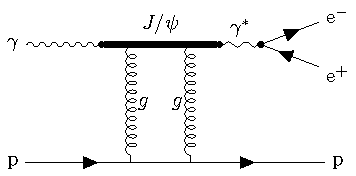
\includegraphics[width=\linewidth]{Figures/Jpsi_FD.pdf}
        \caption{$J/\psi$ photoproduction.}
    \end{subfigure}
    \hspace{0.05\textwidth} % Adjust the length as needed
    \begin{subfigure}{0.22\textwidth}
        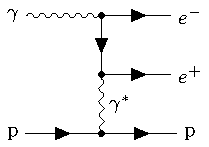
\includegraphics[width=\linewidth]{Figures/BH_FD.pdf}
        \caption{Bethe Heitler process.}
    \end{subfigure}
    \vspace*{-0.0cm}
    \caption{Feynman diagrams illustrating the $J/\psi$ photoproduction
    and the Bethe Heitler process.}
    \label{Fig:Jpsi_BH}
\end{center}
\end{figure}

Figure \ref{Fig:Jpsi_BH} presents the schematic Feynman diagram for the $J/\psi$ photoproduction along with the Bethe-Heitler process. The soft-photon radiation corrections for the Bethe-Heitler process were calculated in \cite{Heller:2018ypa}. These include vertex corrections, lepton self-energy corrections, and real photon emission from the outgoing leptons. Conversely, the $J/\psi$ radiation corrections include only the correction to the $J/\psi$ decay to leptons. These corrections are considered in this paper, see Figure \ref{Fig:Jpsi_RC}.
%%%%%%%%%%%%  J/psi photoproduction RC
\begin{figure}[h]
\begin{center}
    \begin{subfigure}{0.25\textwidth}
        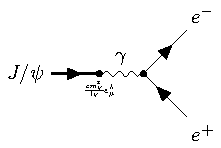
\includegraphics[width=\linewidth]{Figures/born.pdf}
        \caption{Born diagram}
        \label{fig:born}
    \end{subfigure}
    \hspace*{\fill} % separation between the subfigures
    \begin{subfigure}{0.25\textwidth}
        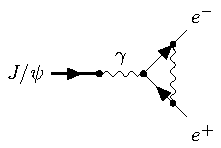
\includegraphics[width=\linewidth]{Figures/vertex.pdf}
        \caption{Vertex correction}
        \label{fig:vertex}
    \end{subfigure}
    \hspace*{\fill} % separation between the subfigures
    \begin{subfigure}{0.35\textwidth}
        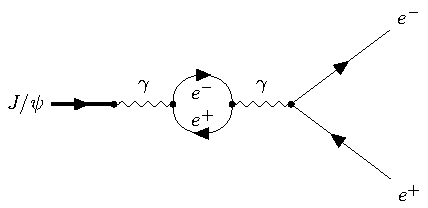
\includegraphics[width=\linewidth]{Figures/vacuom.pdf}
        \caption{Vacuum polarization}
        \label{fig:vacuum}
    \end{subfigure}
    \hspace*{\fill} % separation between the subfigures
    \begin{subfigure}{0.25\textwidth}
        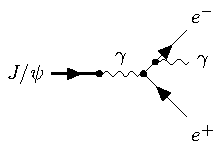
\includegraphics[width=\linewidth]{Figures/brem1.pdf}
        \caption{Bremsstrahlung $e^-$}
        \label{fig:brem1}
    \end{subfigure}
    \hspace*{\fill} % separation between the subfigures
    \begin{subfigure}{0.25\textwidth}
        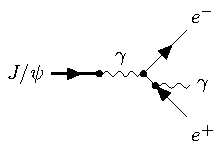
\includegraphics[width=\linewidth]{Figures/brem2.pdf}
        \caption{Bremsstrahlung $e^+$}
        \label{fig:brem2}
    \end{subfigure}
    \vspace*{-0.0cm}
    \caption{Radiative corrections for the $J/\psi \to l^+l^-$ decay.} 
    \label{Fig:Jpsi_RC}
\end{center}
\end{figure}

We can conclude from these considerations that radiative corrections are expected to differ for these particular processes, even in the approximation of soft-photon emission. Numerical calculations support this conclusion. 


%     Vector mesons decay to electron-positron or muon pair
\section{Vector mesons decay to electron-positron or muon pair}
In the framework of the vector-dominance model (VDM) hadron electromagnetic current  reads \cite{Chavin1976}:
\begin{equation}
\braket{V(k),\lambda | j^\mu(0)| 0}=\frac{em_V^2}{f_V}\epsilon^\mu_\lambda(V),
\end{equation}
\noindent
where 
$e$ is the positron charge magnitude ($e^2=4\pi\alpha$),
$m_V$ is a vector meson mass, 
$k_\mu$ is four-momentum of a vector meson,
$\lambda$ is the vector meson's helicity,
$\epsilon^\mu_\lambda$ is the vector meson polarization vector and 
$f_V$ is dimensionless coupling constant. 
The constant $f_V$ is sometimes denote by $2\gamma_V$.The choice of mass in the numerator is arbitrary. It is conventional to choose it as a vector meson mass. 

The vector meson polarization vector $\epsilon_\mu$  is a four-vector that describes the polarization state of a vector meson. 
For a vector meson with mass $m_V$  and four-momentum $p_\mu$ , the polarization vector   satisfies the following properties:
\begin{enumerate}
\item Transversality: $ \epsilon_\mu p_\mu = 0$.
    This means that the polarization vector is orthogonal to the meson's momentum vector.
    
\item Normalization: $ \epsilon_\mu \epsilon^\mu = -1$.
    This normalization condition ensures that the polarization vector is properly normalized. For massive vector mesons, the polarization vector can have different states corresponding to the possible spin projections.
\end{enumerate}
For a vector meson with spin along the direction \(\mathbf{n}\), the polarization vector is given by \(\epsilon^\mu=(0,\mathbf{n})\).

\noindent
The matrix element of the decay $V \to l^+l^-$ of the Born term Figure~\ref{Fig:Jpsi_RC}(a)  reads \cite{Balitsky2024}:

\begin{equation}
{\cal M}~={e^2 m_V^2\over f_V} \epsilon^\lambda_\mu(V){1\over k^2}\bar u \gamma_\mu v~=~{e^2\over f_v}\epsilon^\lambda_\mu(V)\bar u\gamma_\mu v,
\end{equation}
\noindent
and 

\begin{equation}
|{\cal M}|^2~=~{e^4\over f_V^2}\sum_{s_1,s_2}\bar u(p_1,s_1)\slashed{\epsilon}^\lambda v(p_2,s_2)\bar v(p_2,s_2)\slashed{\epsilon}^\lambda u(p_1,s_1),
\end{equation}
\noindent
where $p_1=p_-$ and $p_2=p_+$ are the 4-vectors of leptons and $m$ is the lepton mass.  
In the rest frame of the vector meson $p_1=\big({m_V\over 2},\vec{p}_l\big)$, $p_2=\big({m_V\over 2},-\vec{p}_l\big)$, 
$|\vec{p}_l|~=~{m_V\over 2}\sqrt{1-{4m^2\over m_V^2}}$ and $\epsilon^\lambda\cdot k=m_V\epsilon^\lambda_0=0$.

\begin{equation}
\begin{split}
& \frac{1}{4}\sum_{s_1,s_2}\baru(p_1,s_1)\slashed{\epsilon}^\lambda v(p_2,s_2)\barv(p_2,s_2)\slashed{\epsilon}^\lambda u(p_1,s_1) 
= \frac{1}{4}{\rm Tr}\{\slashed{\epsilon}(\slashed{p} - m)\slashed{\epsilon}(\slashed{p} + m)\} \\
&= 2(p_1 \cdot \epsilon)(p_2 \cdot \epsilon) - \epsilon^2(p_1 \cdot p_2) - m^2 \epsilon^2 
= -2|\vec{p}_1|^2\cos^2{\theta} + \frac{m_V^2}{2} \\
&= \frac{m_V^2}{2} - \frac{m_V^2}{2} \left(1 - \frac{4m^2}{m_V^2}\right) \cos^2{\theta} 
= \frac{m_V^2}{2} \left(\sin^2{\theta} + \frac{4m^2}{m_V^2} \cos^2{\theta}\right)
\end{split}
\end{equation}
%%%%%%%%%%%%%%%%%%%%
Thus, we get
%
\beq
|{\cal M}|^2~=~2m_V^2{e^4\over f_v^2}\Big(\sin^2{\theta}+\frac{4m^2}{m_V^2} \cos^2{\theta}\Big)
\label{Eq:M2}
\eeq
\noindent
The differential decay probability is defined by the equation
\begin{equation}
 d\Gamma=\frac{1}{32\pi^2} | {\cal M}|^2 \frac{|p_l|}{m_V^2}d\Omega = \frac{1}{64\pi^2}\frac{ |{\cal M}|^2}{m_V}\sqrt{1-\frac{4m_l^2}{m_V}} d\Omega.
 \end{equation}
\noindent
 After integrating over $d\Omega=d\phi d\cos{\theta}$ we are getting the total partial width $\Gamma_0(V\to l^-+l^+)$:
\begin{equation}
\Gamma_0(V\to l^-+l^+)=\frac{4\pi\alpha^2}{f_V^2}\frac{m_V}{3} \left(1+\frac{2m_l^2}{m_V^2}\right) \sqrt{1-\frac{4m_l^2}{m_V^2}}.
\end{equation}
\noindent
In the approximation $m_l<<m_V$ the equation simplifies to
\begin{equation}
\Gamma_0(V\to l^-+l^+)=\frac{4\pi\alpha^2}{f_V^2}\frac{m_V}{3}.
\label{Eq:total_width}
\end{equation}
\noindent
The coupling constant $f_V$ is defined directly by the partial decay width $\Gamma_0(V \to l^+l^-)$ in Eq.~\ref{Eq:total_width}.
The vector-dominance model constants $f_V$ are listed in Table~\ref{Table:1}.

\begin{table}[h!]
\centering
\caption{Vector Dominance Model Constants }
\begin{tabular}{|c|c|c|c|c|c|}
\hline
                      & Mass& Full Width $ \Gamma_0$ & $BR(V\to e^+e^-)$ & $\Gamma(V\to e^+e^-)$ & $f_V$ \\
                      & MeV & MeV                                 &                      & MeV                              &          \\
\hline
\hline
$\rho(770)$     & 775.96 & 149.1                                & 4.72e-5                  & 7.04e-3 & 4.96 \\
\hline
$\omega(782)$ &782.66 & 8.68                                &   7.38e-5               &  6.41e-4& 16.5 \\
\hline
$\phi(1020)$    & 1019.46 & 4.249                                & 2.979e-4                & 1.27e-3 & 13.4 \\
\hline
$J/\psi(1S)$ & 3096.9 & 0.0926                               & 5.971e-2                  & 5.53e-3 & 11.18 \\
\hline
\end{tabular}
\label{Table:1}
\end{table}


 %  Section Radiation Corrections
\section{Radiation Corrections}
The first-order QED  radiation corrections to the width of the vector meson $V\to l^+l^-$ decay, electrons and muons, were calculated a while ago in \cite{Ehlotzky1968}.

The total width $\Gamma(V \to l^+l^-)$ with the radiative corrections reads
\begin{equation}
\Gamma = \Gamma_0(1+\delta_S+\delta_H),
\end{equation}
\noindent
where $\Gamma_0$ is the Born term total width (Figure~\ref{fig:born}),  $\delta_S$ stands for the soft-photons radiative corrections determined by diagrams in Figures~\ref{fig:vertex}-\ref{fig:brem2} as well as of real photons whose energy is less a cut-off energy ${E_\gamma<\varepsilon}$, 
and  $\delta_H$ accounts for the emission of the hard bremsstrahlung photons with the energy  ${E_\gamma>\varepsilon}$. The corrections to the total width 
$\Gamma$ define actually radiative corrections for the cross section of the photoproduction process
$\gamma p \to J/\psi p \to l^+l^- p$
\begin{equation}
\sigma = \sigma_0(1+\delta_S+\delta_H).
\end{equation}
\noindent

It is important to understand that all the above-mentioned amplitudes, except Born and
vac, contain infrared-divergent terms (tending to infinity in the limit of very soft, or
‘infrared’, photons). These are canceled out completely in the sum of all diagrams in Figure\ref{Fig:Jpsi_RC}(b)-(e), which is therefore
finite. More precisely, there are the following cancellations of the infrared divergences: between the lepton vertex correction and the lepton bremsstrahlung
correction. The vacuum polarization corrections, shown in Figure \ref{Fig:Jpsi_RC}(c), is finite.
It is convenient to separate the amplitude into ‘soft’ and ‘hard’ parts,
The label ‘soft’ implies the assumption that at least
one virtual photon is soft. Infrared divergences are completely
contained in the soft part. 
 
It is important to understand that first-order bremsstrahlung is taken into
account in both cases, and the separation between these two types of events is based on the
energy of the emitted photon. If this energy does not exceed the cut-off value $E_\gamma^{cut}<\varepsilon$ (which can
be set to, for example, 1 MeV for the experiments of interest), then the process can
be effectively considered as pure $\gamma p\to J/\psi p\to l^+l^-p$ without bremsstrahlung photons since the experiment can not distinguish it from the  
$\gamma p\to J/\psi p\to l^+l^-p \gamma$ process. In this case, it is not necessary to consider such soft photons in the Monte
Carlo simulation, so we can analytically integrate the cross section of the first-order bremsstrahlung $\gamma  p\to J/\psi p\to l^+l^-p \gamma$ 
process over all directions of the emitted photon and over its energy in
the range $E_\gamma<\varepsilon$. Moreover, we can confidently use the primary soft-photon approximation
to perform this integration, because it works well for very low-energy photons. 

The quantity $\delta=\delta_S+\delta_H$
includes both the corrections due to the emission of a real bremsstrahlung photon and the
virtual-photon corrections. However, corrections of both these types are
infrared-divergent, so that only the total correction $\delta$ can be defined uniquely. The only
exception is the vacuum polarization correction $\delta_{vacuum}$, which is finite and therefore can be
determined individually.

%%%%%%%%%%%%%%%%%%%%%%%%%%%%%%%%%%%%%%%%%
\section{Soft Radiation Corrections}
In any experiment with finite energy resolution, the emission of additional soft photons with $|k|<\varepsilon$  is undetectable and
thus gets subsumed in the cross section for the elastic scattering process. 
The integrals  over a (small) momentum sphere 
$|k|<\varepsilon$ are shown in Eq. \ref{Eq:deltaSe} for electrons and in Eq. \ref{Eq:deltaSmu} for muons \cite{Ehlotzky1968}:


%%%% Eq. Soft energy RC electrons
\begin{equation}
\delta_S(M_V,\varepsilon) = -\frac{4\alpha}{\pi} \left[   \left( \ln\frac{M_V}{m_e}-\frac{1}{2}\right)  \left(\ln\frac{M_V}{2\varepsilon}-\frac{13}{12} \right)+\frac{17}{72}- \frac{\pi^2}{12} \right].
\label{Eq:deltaSe}
\end{equation}
\noindent

%%%% Eq. Soft energy RC muons
\begin{equation}
\delta_S(M_V,\varepsilon) = -\frac{4\alpha}{\pi} \left[   \left( \ln\frac{M_V}{m_\mu}-\frac{1}{2}\right)  \left(\ln\frac{M_V}{2\varepsilon}-\frac{13}{12} \right)+\frac{17}{72}- \frac{\pi^2}{12}   
+\left( \frac{5}{18}-\frac{1}{3}\ln\frac{M_V}{m_e}\right) \right].
\label{Eq:deltaSmu}
\end{equation}
\noindent
Soft photon limit is defined by a scaling of the momenta of virtual photons in the loops and real photons momenta in the bremsstrahlung process, with respect to external scales. 

Soft radiative corrections $\delta_S$ for electrons and muons as a function $\varepsilon$ are presented in Figure \ref{Fig:delta_soft}.
%FIG. soft muons
\begin{figure}[h]
\begin{center}
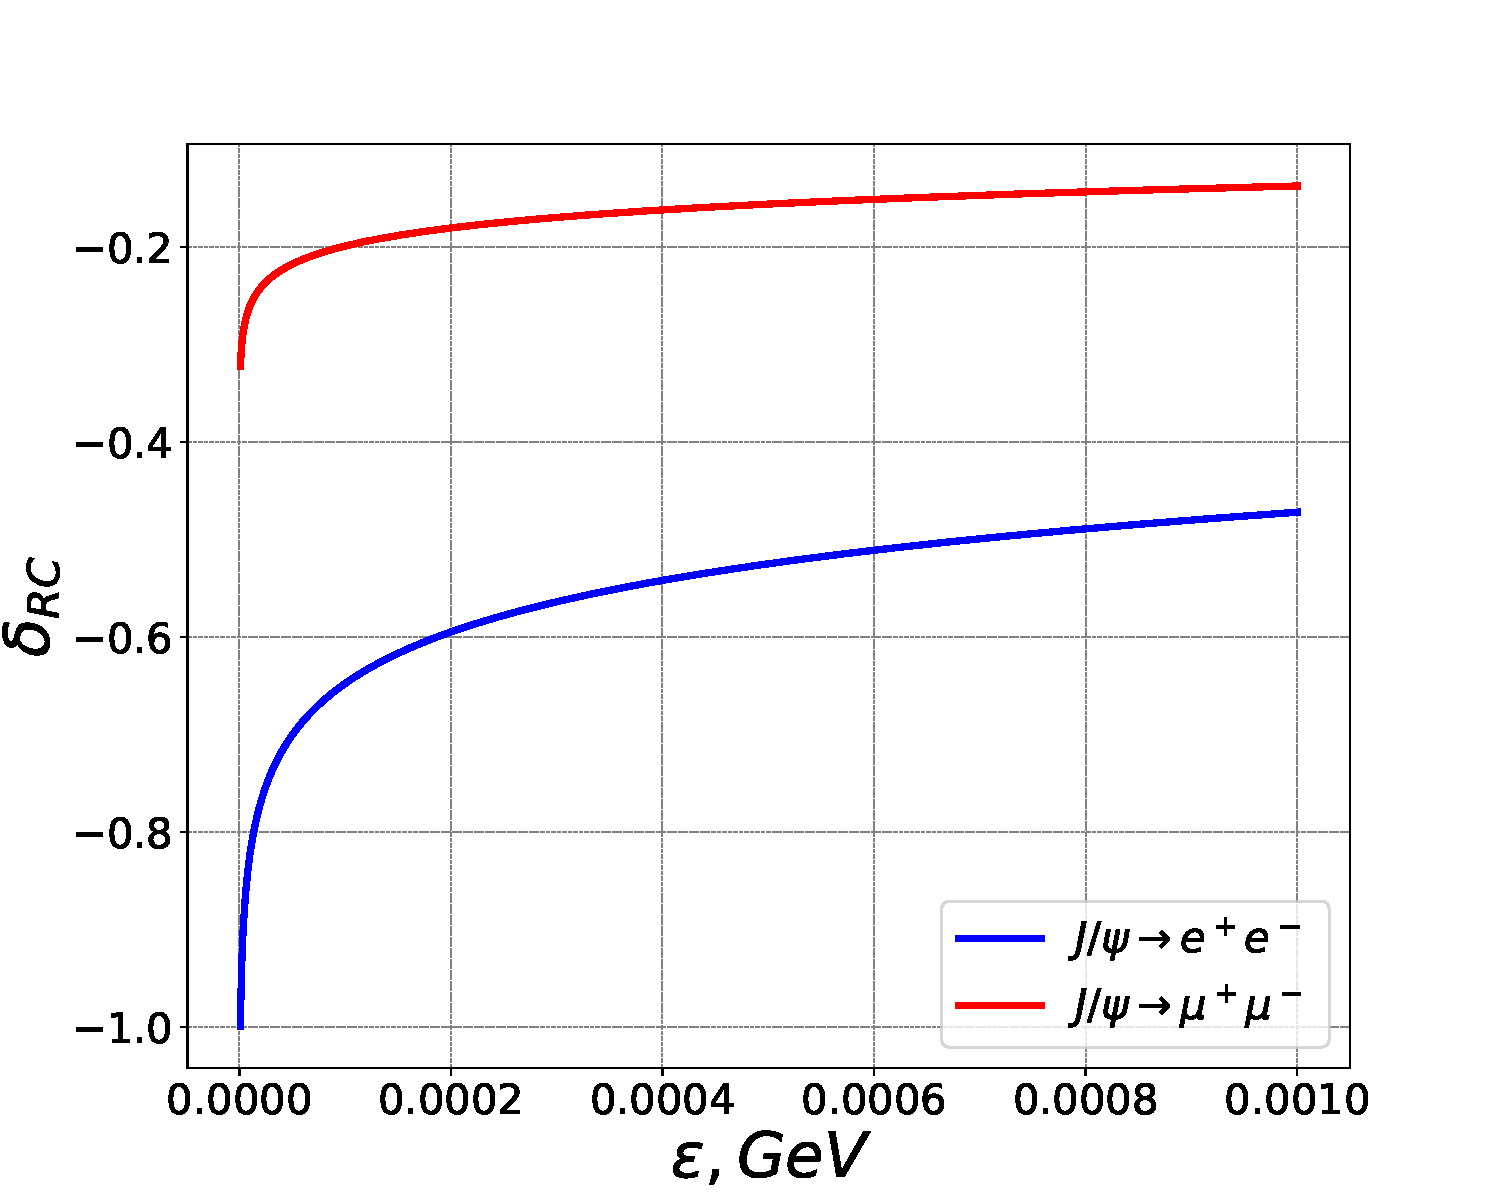
\includegraphics[width=0.5\textwidth]{Figures/soft_RC.pdf}
\vspace*{-0.0cm}
\caption{Soft radiative corrections $\delta_S(M_{J/\psi},\varepsilon)$ as a function $\varepsilon$.}
\label{Fig:delta_soft}
\end{center}
\end{figure}



%%%%%%%%%%%%%%%%%%%%%%%%%%%%%%%%%%%%%%%%%
\section{Hard Radiation Corrections}

The exact calculation of the hard radiative corrections $\delta_H$ would require a rather complicated angular integration of the decay probability. At high energy it could be done in the peaking approximation when additional hard photon is emitted parallel to the lepton (or antilepton) momentum. According to \cite{Kessler1960} and \cite{Longhi1965} we get
%%%%  dN/dk

\begin{equation}
\frac{d\Gamma_H}{dk} =\Gamma_0 \frac{2\alpha}{\pi} \left[ 2\ln{ \left( \frac{M_V}{m_e} \sqrt{1 - \frac{2k}{M_V}} \right) - 1} \right] \frac{1}{k}\left(1-\frac{2k}{M_V}+\frac{2k^2}{M_V^2} \right).
\label{Eq:dNdk}
\end{equation}
\noindent
The integration of Eq. \ref{Eq:dNdk} in the range of the photon energy $(\varepsilon, k_{max})$ is presented 
in Eq. \ref{Eq:harde} for electrons and Eq. \ref{Eq:hardmu} for muons. 
%%%% Eq. hard energy RC electrons
\begin{equation}
\delta_H(M_V,\varepsilon,k_{max}) = -\frac{4\alpha}{\pi} 
\left[
   \left( \ln\frac{M_V}{m_e}-\frac{1}{2}\right)  \left( \ln\frac{\varepsilon}{k_{max}}+\frac{3}{4} \right)+\frac{1}{2}L_2(r_{max}) + R(r_{max})  + \frac{r_{max}^2}{16}-\frac{3}{8}r_{max}
\right] 
\label{Eq:harde}
\end{equation}
\noindent

%%%% Eq. hard energy RC muons
\begin{equation}
\delta_H(M_V,\varepsilon,k_{max}) = -\frac{4\alpha}{\pi} 
\left[
   \left( \ln\frac{M_V}{m_\mu}-\frac{1}{2}\right)  \left( \ln\frac{\varepsilon}{k_{max}}+\frac{3}{4} \right)+\frac{1}{2}L_2(r_{max}) + R(r_{max})  + \frac{r_{max}^2}{16}-\frac{3}{8}r_{max}
\right] 
\label{Eq:hardmu}
\end{equation}
\noindent

%%%% Eq. r_max
\begin{equation}
r_{max} = \frac{2k_{max}}{M_V}
\label{Eq:rmax}
\end{equation}
\noindent

%%%% L_2(x)
\begin{equation}
L_2(x)= -\int^x_0\frac{\ln(1-t)}{t}dt
\label{Eq:L2}
\end{equation}
\noindent

%%%%  R(rmax)
\begin{equation}
\begin{split}
&R(r_{max}) = \left(r_{max}-\frac{r_{max}^2}{4}-\frac{3}{4}\right)\left[  \ln {\left(\frac{M_V}{m_e}\sqrt{1-r_{max}}\right)} -\frac{1}{2}\right],\\
&R(r_{max}=1)=0,~~~~~L_2(r_{max}=1)=\frac{\pi^2}{6}
\end{split}
\end{equation}
\noindent
%FIG. dNdk0 muons and electrons
\begin{figure}[h]
\begin{center}
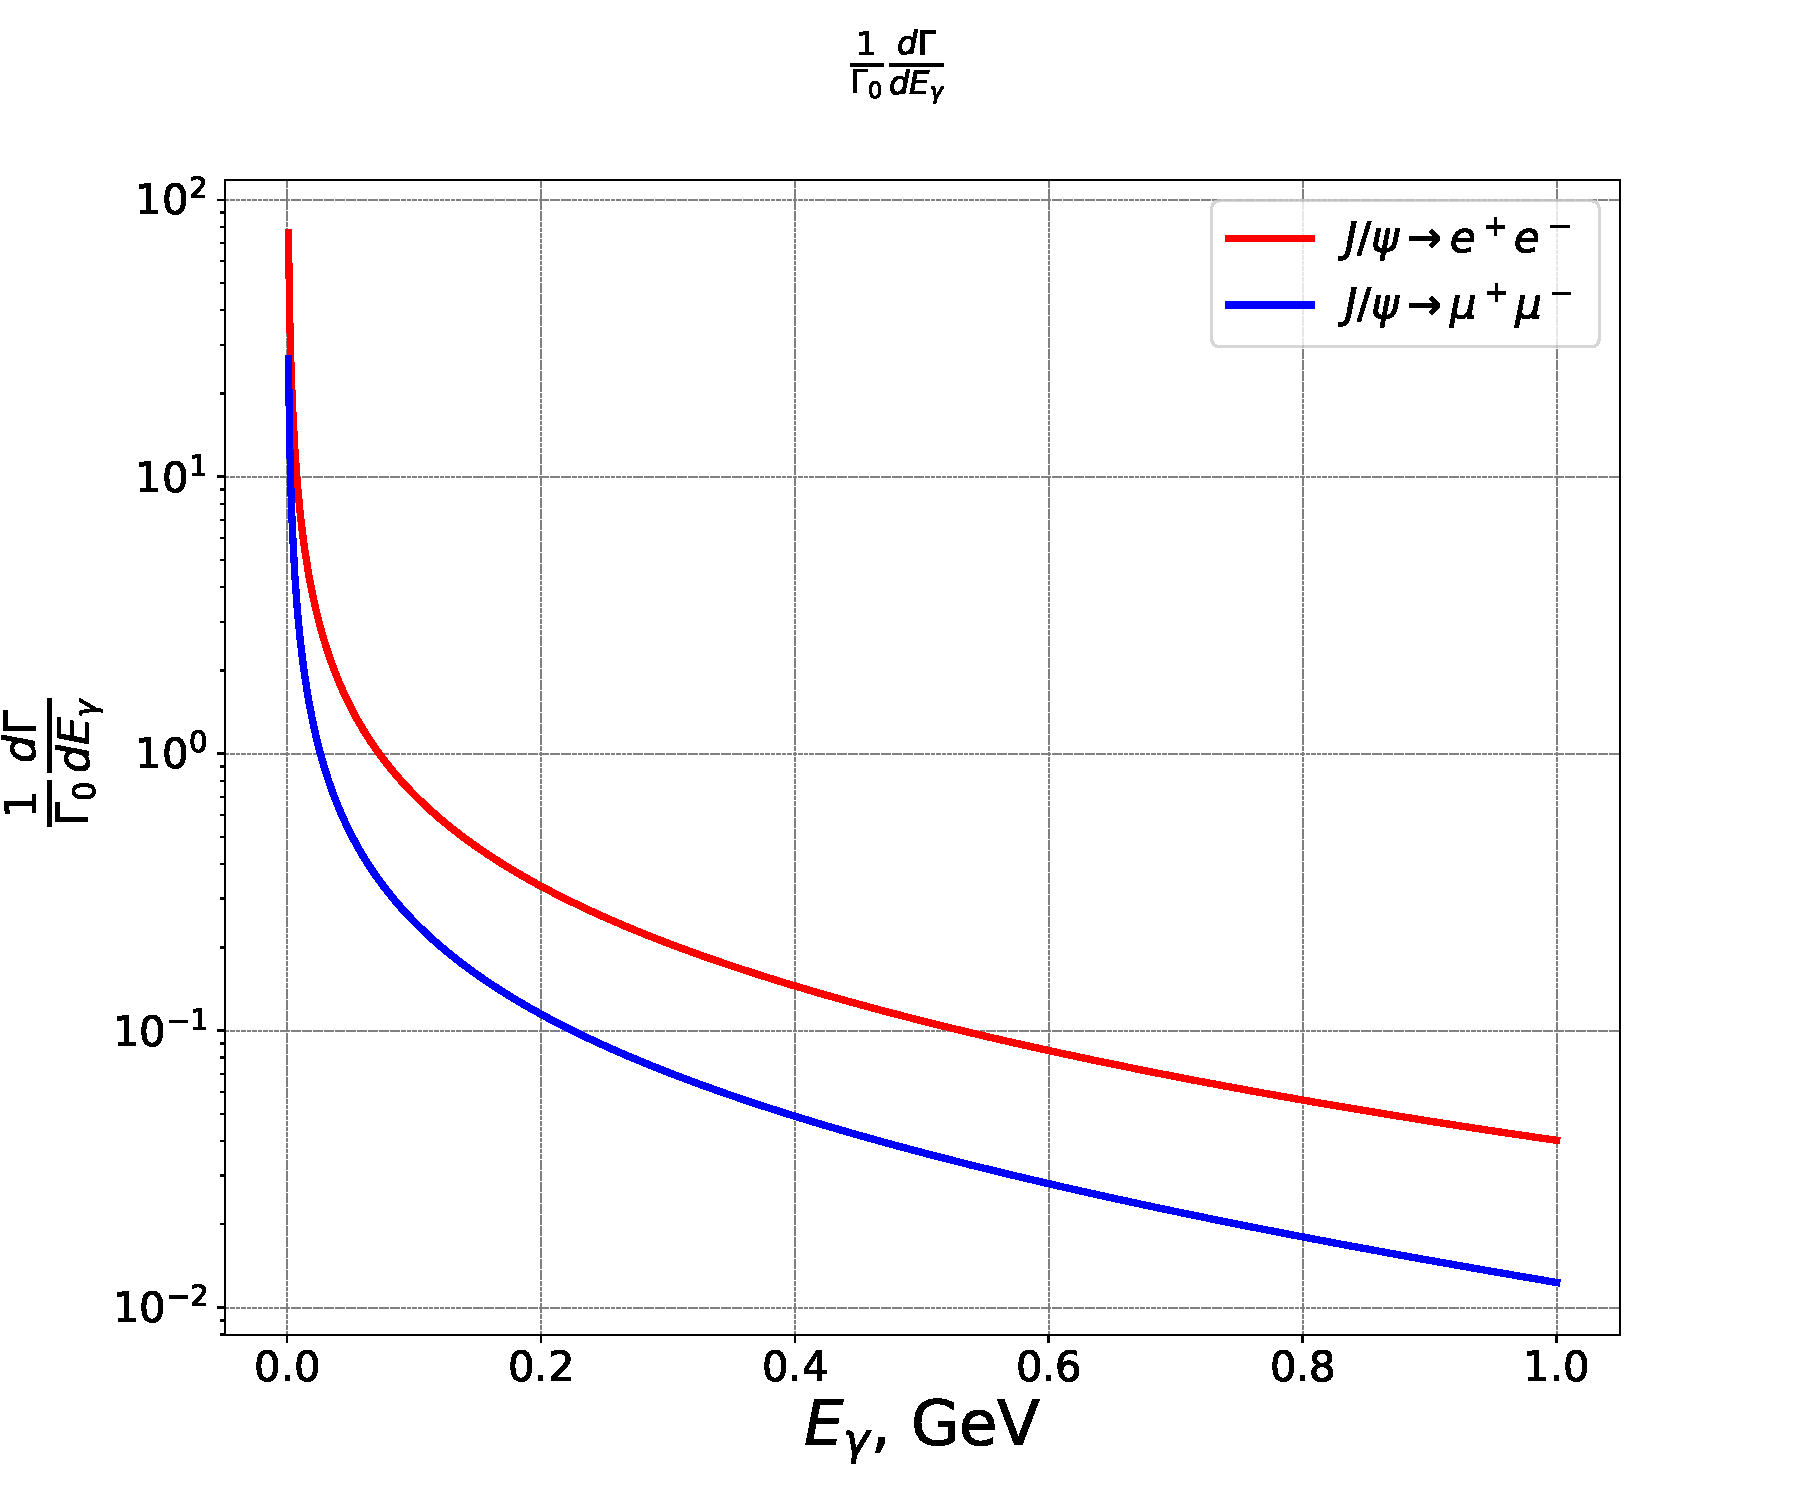
\includegraphics[width=0.5\textwidth]{Figures/dNdk0_e_mu.pdf}
\vspace*{-0.0cm}
\caption{Hard  photon energy distribution for electrons and muons.}
\label{Fig:dNdk0_mu}
\end{center}
\end{figure}

%FIG. dNdk0
\begin{figure}[h]
\begin{center}
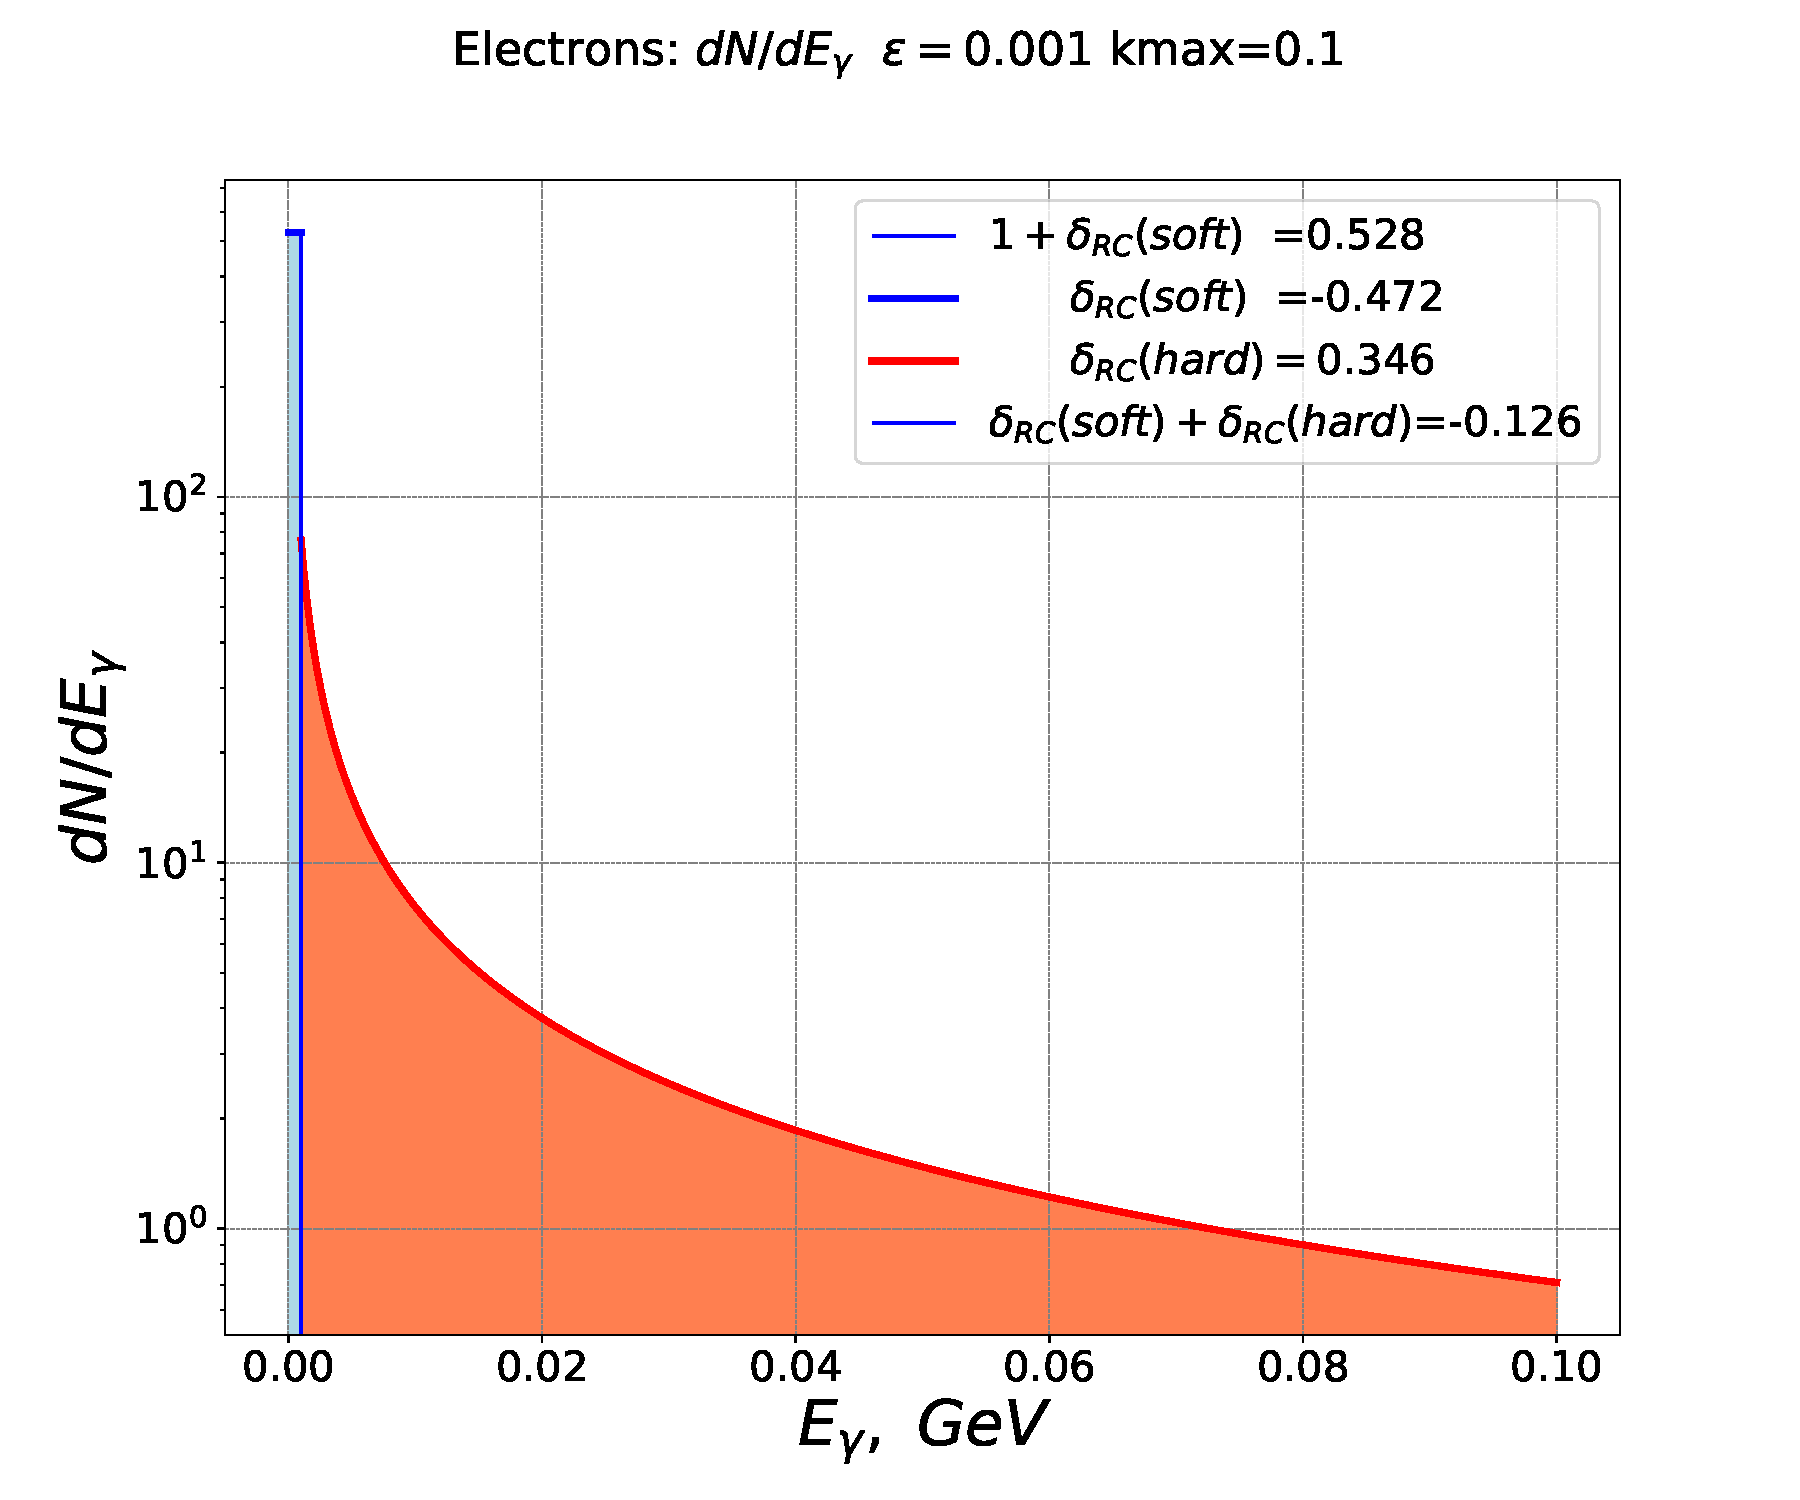
\includegraphics[width=0.5\textwidth]{Figures/dNdk0_HR_kmax_0.1.pdf}
\vspace*{-0.0cm}
\caption{Radiative photon energy distribution for $\varepsilon$=0.001 GeV and $k_{max}$=0.1 GeV. The calculation is done for $J/\psi\to e^+e^-$ decay.}
\label{Fig:dNdk0_s_h}
\end{center}
\end{figure}
The $k_{max}$ photon energy depends on the experimental cut off energy and maximum value is $k_{max}=\frac{M_V}{2}$.
Hard photon energy distributions for electrons and muons are presented in Figure \ref{Fig:dNdk0_mu}.

The energy distribution  for $\varepsilon$=0.001 GeV and $k_{max}$=0.1 GeV parameter set is presented in Figure \ref{Fig:dNdk0_s_h}.
The blue curve is for soft photons $E\gamma<\varepsilon$ and red curve for hard photons $\varepsilon<E\gamma<k_{max}$.

Hard radiative corrections $\delta_H(M_{J/\psi}, \varepsilon,k_{max})$ as a function of $k_{max}$ with $\varepsilon$=0.001 GeV is presented in Figure \ref{Fig:delta_hard}.
%FIG. hard muons
\begin{figure}[h]
\begin{center}
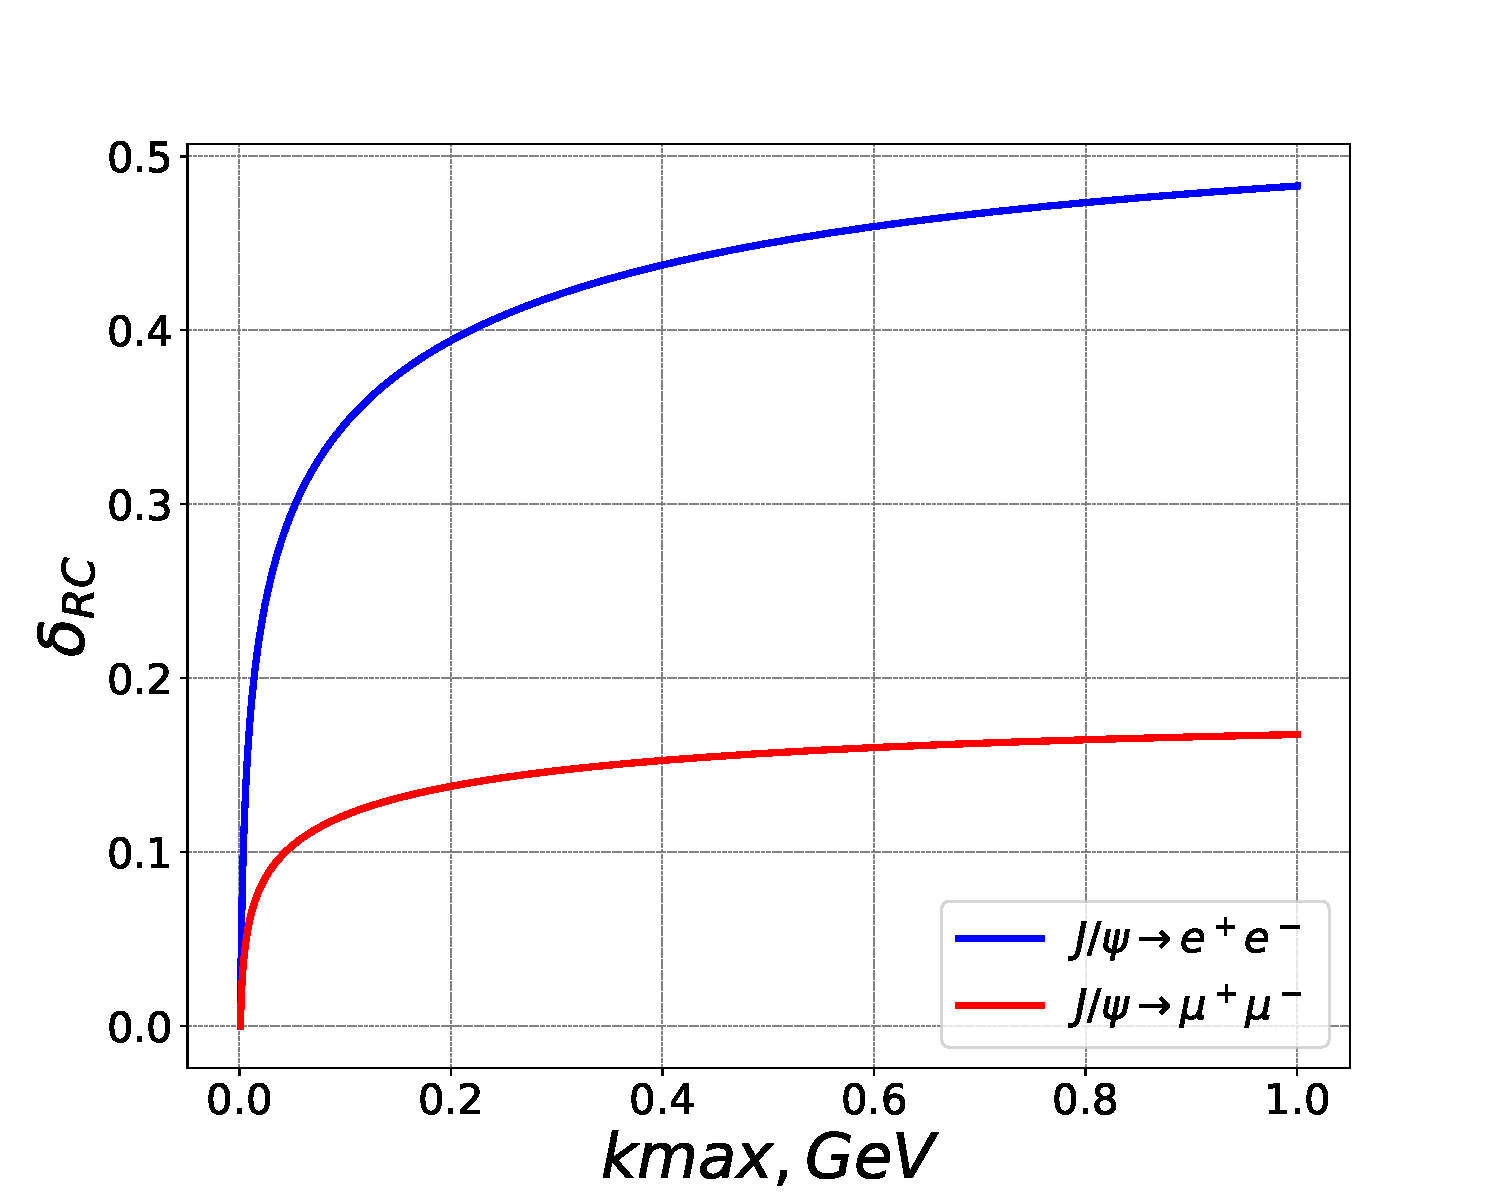
\includegraphics[width=0.5\textwidth]{Figures/hard_RC.pdf}
\vspace*{-0.0cm}
\caption{Hard radiative corrections $\delta_H(M_{J/\psi}, \varepsilon,k_{max})$ as a function of $k_{max}$ with $\varepsilon$=0.001 GeV.}
\label{Fig:delta_hard}
\end{center}
\end{figure}

%%%%%%%%%%%%%%%%%%%%%%%%%%%%%%%%%%%%%%%%%
\section{Total Radiation Corrections}
The total radiative corrections, $\delta(k_{max})=\delta_S(M_V,\varepsilon)+\delta_H(M_V,\varepsilon,k_{max})$ does not depend 
on the $\varepsilon$ any more.
Eq. \ref{Eq:deltaTe} presents total corrections for electrons and Eq. \ref{Eq:deltaTmu} for muons
%%%%  \delta = \delta_V+\delta_R
\begin{equation}
\begin{split}
\delta(M_V,k_{max})=\delta_S+\delta_H  &= -\frac{4\alpha}{\pi}  \left[  \left( \frac{1}{2}-\ln\frac{M_V}{m_e} \right)  \left( \ln r_{max}+\frac{1}{3} \right) \right. \\
                                & \qquad \left.   + \frac{1}{2}\left( L_2(r_{max})-\frac{\pi^2}{6} \right)  +\frac{17}{72}+R(r_{max}) + \frac{r_{max}^2}{16}-\frac{3}{8}r_{max}  \right] \end{split}
\label{Eq:deltaTe}
\end{equation}
\noindent

\begin{equation}
\begin{split}
\delta(M_V,k_{max})=\delta_S+\delta_H  &= -\frac{4\alpha}{\pi}  \left[  \left( \frac{1}{2}-\ln\frac{M_V}{m_\mu} \right)  \left( \ln r_{max}+\frac{1}{3} \right) \right. \\
                                   &\qquad \left. + \frac{1}{2}\left( L_2(r_{max})-\frac{\pi^2}{6} \right)  +\frac{17}{72}+\left( \frac{5}{18}-\frac{1}{3}\ln\frac{M_V}{m_e}\right)+ R(r_{max}) + \frac{r_{max}^2}{16}-\frac{3}{8}r_{max}  \right] \end{split}
\label{Eq:deltaTmu}
\end{equation}
\noindent

Soft, hard and total radiative corrections as a function of the vector meson mass ($\varepsilon$=0.001 GeV, $k_{max}$=0.1 GeV) are presented in Figure \ref{Fig:delta_Mv}.
%FIG. delta vs MV
\begin{figure}[h]
\begin{center}
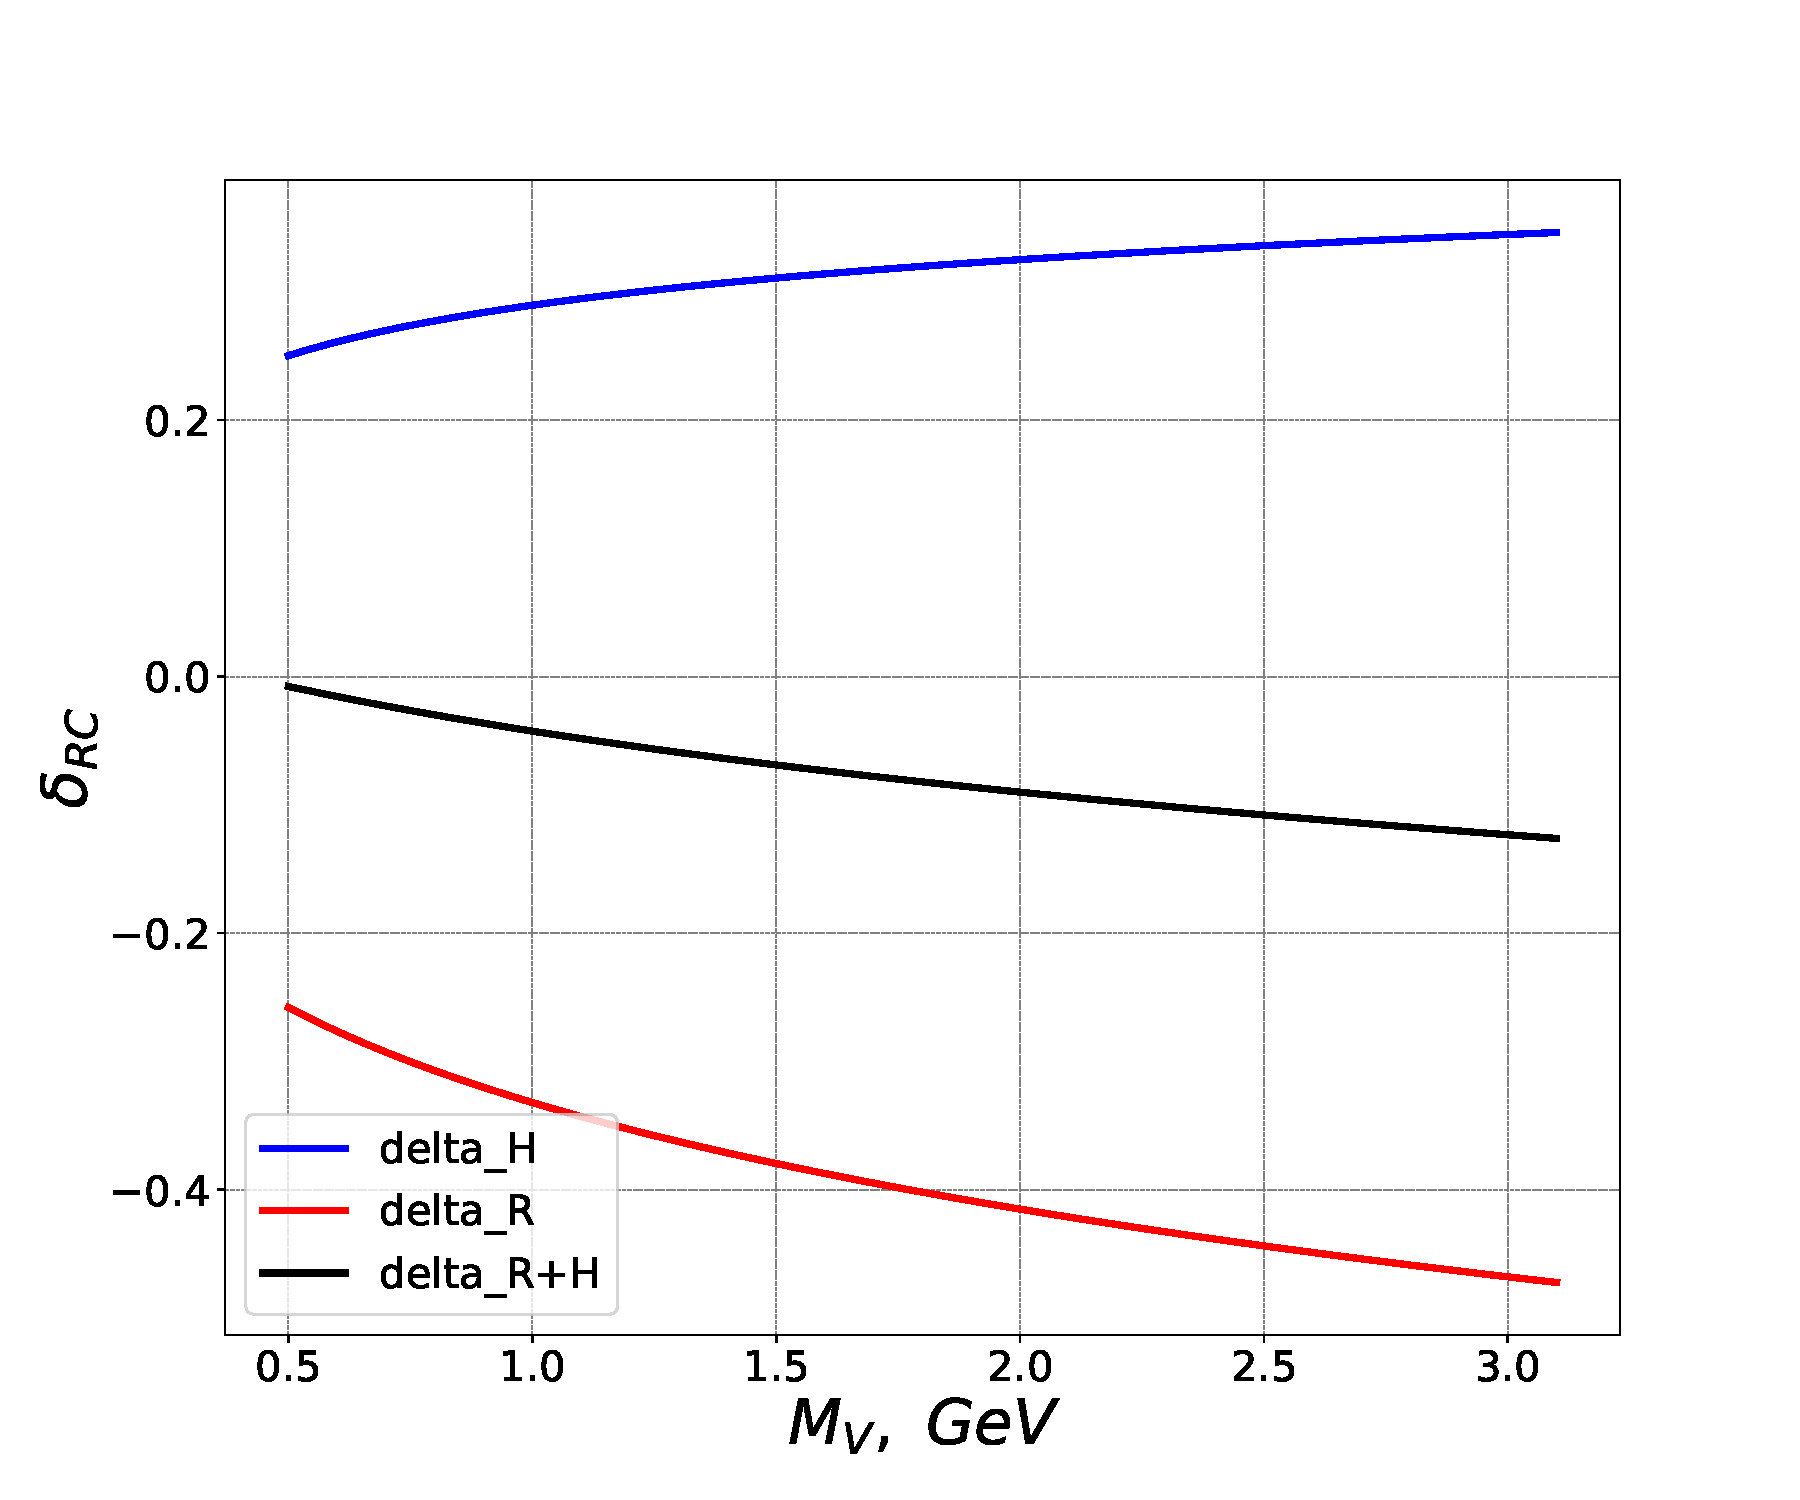
\includegraphics[width=0.5\textwidth]{Figures/RC_Mv_VM.pdf}
\vspace*{-0.0cm}
\caption{Soft, hard and total radiative corrections as a function of the vector meson mass, $\varepsilon$=0.001 GeV and $k_{max}$=0.1 GeV.}
\label{Fig:delta_Mv}
\end{center}
\end{figure}

Total radiative corrections as a function of $k_{max}$ for electrons and muons are presented in Figure \ref{Fig:dNdk0_total}.
%FIG. delta 
\begin{figure}[h]
\begin{center}
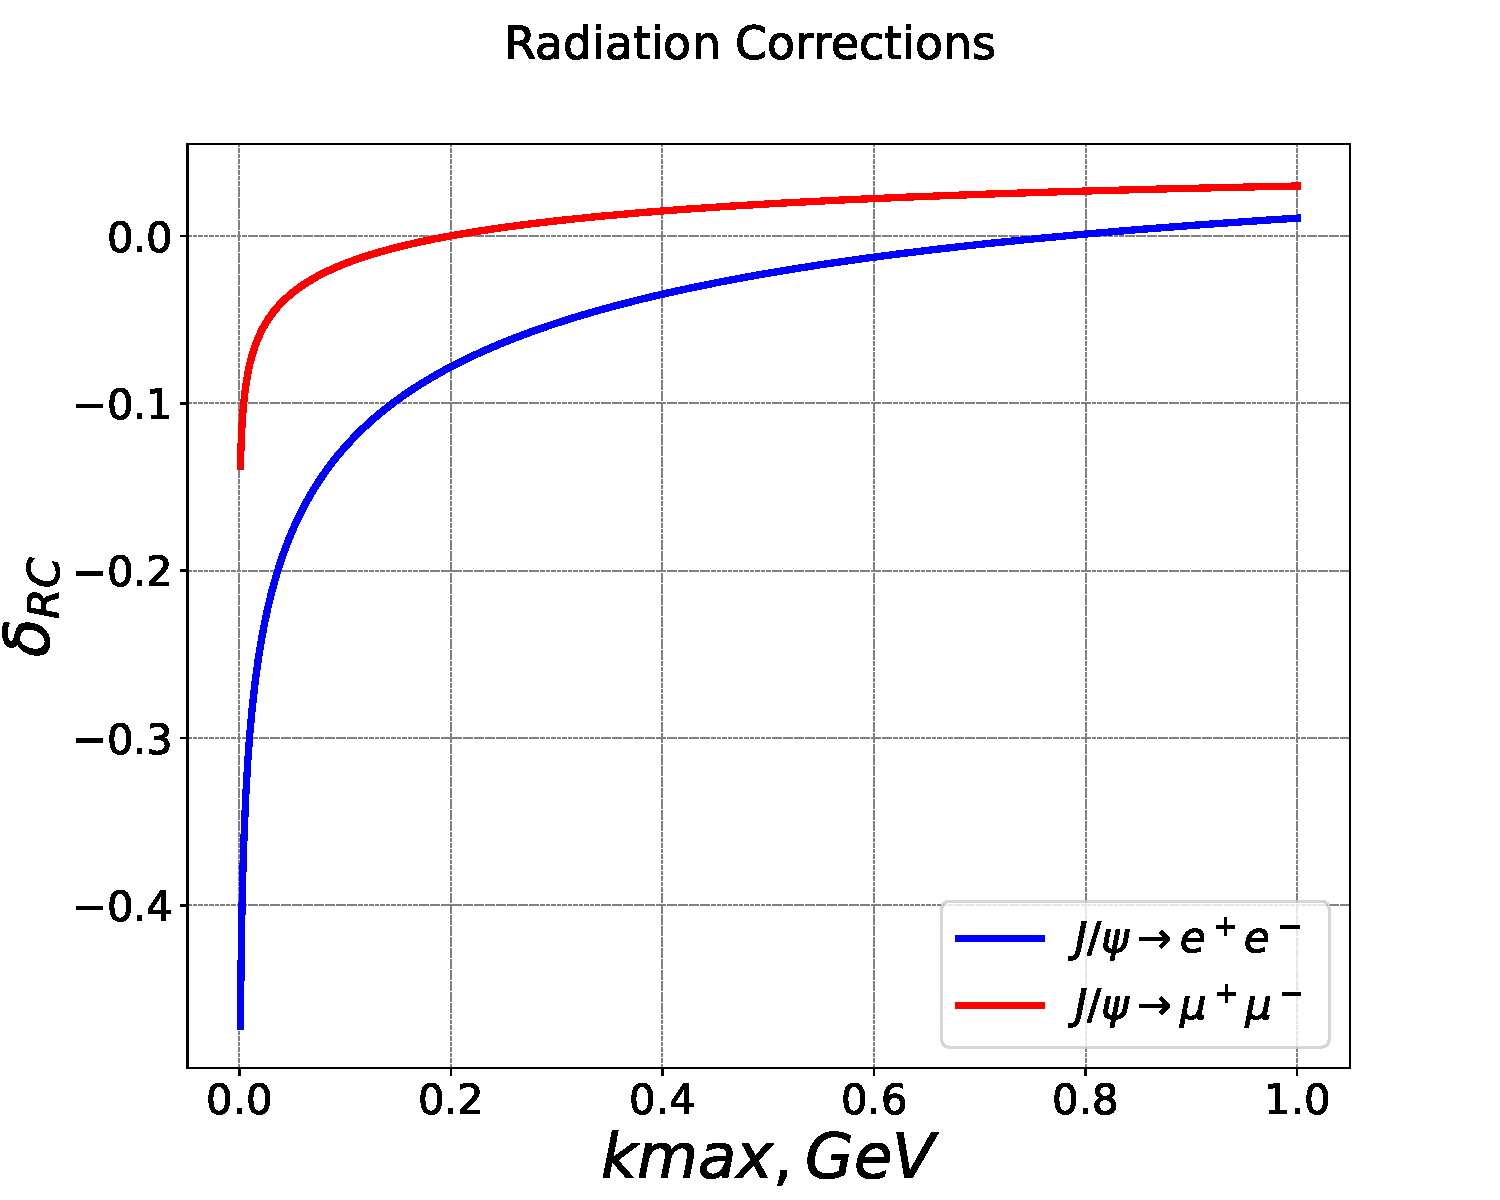
\includegraphics[width=0.5\textwidth]{Figures/HR_RC.pdf}
\vspace*{-0.0cm}
\caption{Total radiative corrections as a function of $k_{max}$ for electrons and muons.}
\label{Fig:dNdk0_total}
\end{center}
\end{figure}



%%%%%%%%%%%%%%%%%%%%%%%%%%%%%%%%%%%%%%%%%
\section{Comparison of the Soft Radiation Corrections for the Vector mesons photoproduction and  Bethe-Heitler processes}
%Comparison
Comparison of the soft radiative corrections for Bethe Heitler (BH) process \cite{Heller:2018ypa} with $M_{e^+e^-}=M_{J/\psi}$ and $J/\psi$ photoproduction \cite{Ehlotzky1968} is presented in Figure \ref{Fig:compar}.  At typical cut-off soft photons energy ${\varepsilon}=0.1~GeV$
$\delta_{RC}(BH)=-20\%$ and $\delta_{RC}(J/\psi)=-12\%$.
\begin{figure}[h]
\begin{center}
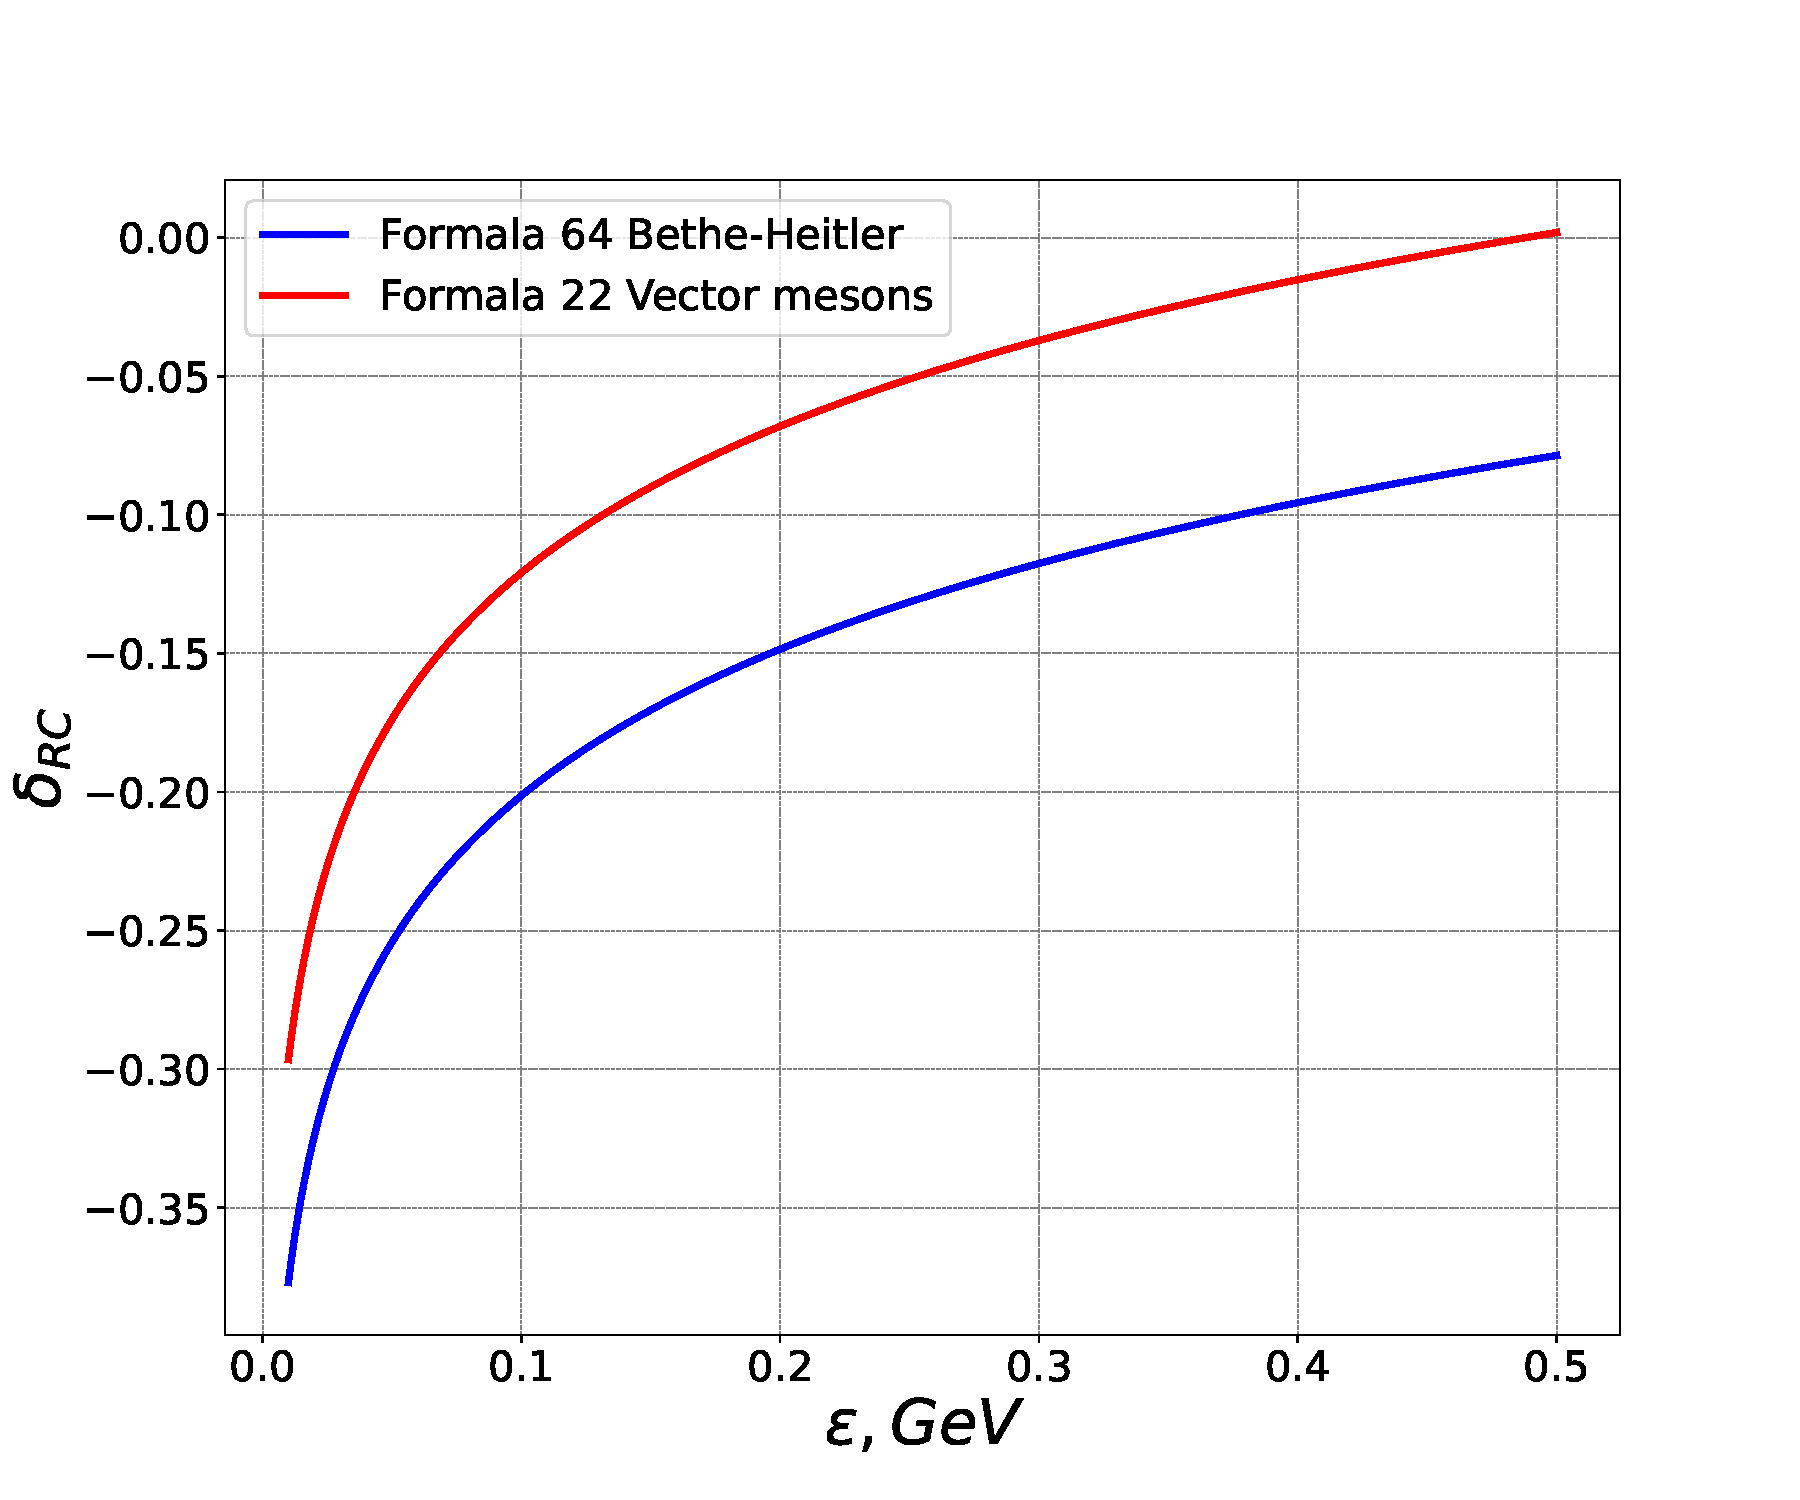
\includegraphics[width=0.5\textwidth]{Figures/RC_VM_BH.pdf}
\vspace*{-0.0cm}
\caption{Comparison of radiative corrections for Bethe Heitler process \cite{Heller:2018ypa} with $M_{e^+e^-}=M_{J/\psi}$ and $J/\psi$ photoproduction \cite{Ehlotzky1968}.}
\label{Fig:compar}
\end{center}
\end{figure}

%%%%%%%%%%%%%%%%%%%%%%%%%%%%%%%%%%%%%%
\section{Invariant mass}
The radiation of the hard photons affects the invariant mass $M_{e^+e^-}$ distribution in the decay $J/\psi\to e^+e^-\gamma$. The calculation of the radiation corrections depends on the maximum energy of the photon $k{max}$. In the $J/\psi$ center of mass the energy of the photon is directly connected with the $M_{e^+e^-}$ measured in the experiment
\begin{equation}
E_\gamma = \frac {M_{J/\psi}^2-M^2_{e+e-}} {2M_{J/\psi}}.
\label{Eq:Egamma}
\end{equation}
It means that we can use cut on the $M_{e^+e^-}$ to calculate radiation corrections in Eq.~\ref{Eq:harde}-\ref{Eq:hardmu} instead of the maximum energy of the radiated photon, $k_{max}=E_\gamma$.
In the real experiment we study $M_{e+e^-}$ near the $J/\psi$ signal, $M_{e^+e^-}\sim M_{J/\psi}$. In this case we can simplify the equation 
\begin{equation}
E_\gamma = \frac {M_{J/\psi}^2-M^2_{e+e-}} {2M_{J/\psi}}=\frac {(M_{J/\psi}-M_{e+e-})(M_{J/\psi}+M_{e+e-})} {2M_{J/\psi}}\approx M_{J/\psi}-M_{e^+e^-}.
\label{Eq:deltaM}
\end{equation}
It means that the parameter $k_{max}=(M_{J/\psi}-M_{e^+e^-})$ in Eq.~\ref{Eq:harde}-\ref{Eq:hardmu}.
\noindent








%\clearpage 
\section{Summary}

\section*{Acknowledgements}
V.K. acknowledges I. Balitsky, I. Akushevich, and A. Ilyichev for useful discussions, and
support from the U.S. Department of Energy, Office of Science, Office of Nuclear Physics under contracts DE-AC05-06OR23177. JLAB-PHY-22-3641.  
\bibliographystyle{elsarticle-num-names}
\bibliography{Jpsi_RC}
\clearpage
\end{document}
